%\chapter*{Введение}
%\addcontentsline{toc}{chapter}{Введение}

\newpage
\begin{center}
\textbf{ГЛАВА 2}\\
\textbf{ФАЗОВЫЕ ДИАГРАММЫ ПРИ РАЗЛИЧНЫХ ПОТЕНЦИАЛАХ ВЗАИМОДЕЙСТВИЯ}
\end{center}
\refstepcounter{chapter}


% \section*{}
\addcontentsline{toc}{chapter}{ГЛАВА 2. Фазовые диаграммы при различных потенциалах взаимодействия}
\section{Метод построения фазовых диаграмм с помощью разбиения на ячейки вороного}\label{C2_1}

Метод построения фазовых диаграмм с помощью разбиения на ячейки вороного, введенный в статье \cite{Ovcharov2017}, основан на триангуляции Делоне и разбиении систем частиц на ячейки Вороного, для последующего их анализа.

Построив гистограмму вороного для множества точек, каждой точке можно сопоставить ряд параметров:
\begin{itemize}
\item Площадь и плотность ячейки.
\item Число граней каждой ячейки, каждая из которых принадлежит ячейке "соседу" (далее будет использован термин \textbf{соседняя частица}).
\item Параметр порядка и т.д.
\end{itemize}
Плотность ячейки вороного будет рассчитываться как величина, обратная площади:
\begin{equation}
\rho_i = 1 / S_i,
\label{eqRho}
\end{equation}
где $\rho_i$ - плотность соответствующей частицы, $S_i$ - ее площадь.

\begin{figure}[h]
\begin{center}
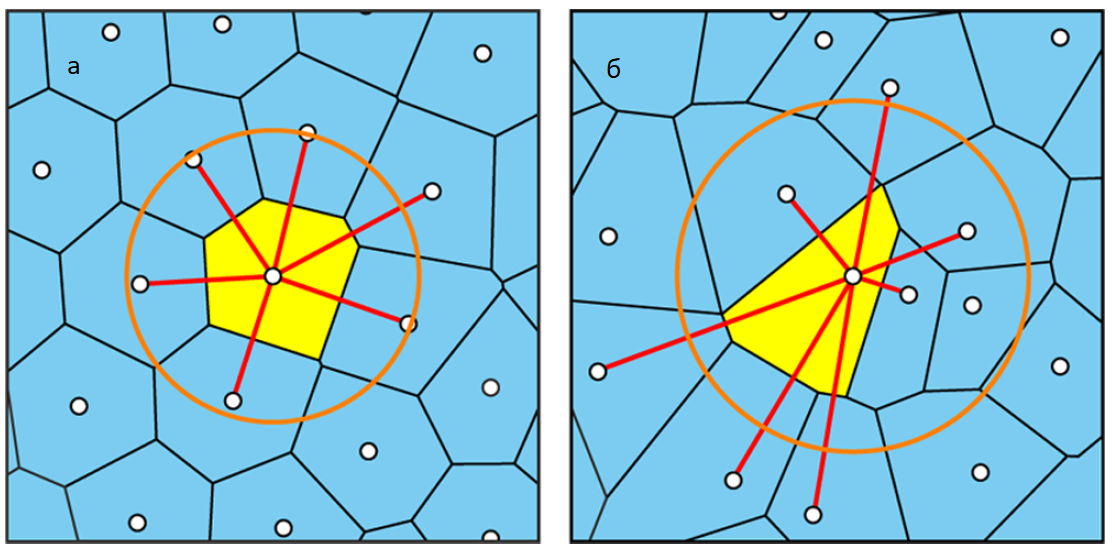
\includegraphics[width=0.7\textwidth]{rgcell}
\caption{Пример разбиения на ячейки вороного в конденсированном кластере (а) и газе (б). Частицы представлены белыми точками, а ячейки, соответствующие рассматриваемым частицам раскрашены в желтый цвет. Радиус окружностей соответствует среднему расстоянию между частицей и ее соседями.}
\label{risFlucMed}
\end{center}
\end{figure}

На рисунке \ref{risFlucMed} показана часть $2D$ - системы, полученной с использованием МД-моделирования потенциала Леннарда-Джонса (LJ12-6 при плотности частиц $n_0 = 0.4$).
Сравнивая ячейки вороного в конденсированной среде и газе можно заметить, что конденсированное состояние отличается меньшей площадью частиц. Из-за большей плотности частиц в конденсате, расположение частиц сильно ограниченно, вследствие чего ячейки получаются более правильной формы. Это дает возможность ввести некоторую величину, которая будет показывать отклонение от правильной формы.

\begin{equation}
	R_{0i} = \sqrt{\frac{\pi}{2 S_i N_{ni}^2} \sum\limits_{i<k}^{N_{ni}} (r_{ij} - r_{ik})^2}, r_{ij} = |r_i - r_j|,
\end{equation}

где $S_i$ - площадь рассматриваемой частицы; $N_{ni}$ - количество соседей частицы; $r_{ij}$ - расстояние от рассматриваемой частицы до соседней.
Для уменьшения сильных колебаний величины $R_{0i}$, она усредняется по соседним частицам:

\begin{equation}\label{eqIrreg}
R_i = \frac{1}{N_{ni} + 1} \left( R_{0i} + \sum\limits_{j=1}^{N_{ni}} R_{0j} \right),
\end{equation}

где $R_{0i}$ - неусредненный параметр искомой частицы, рассчитанный по формуле \ref{eqIrreg}; $R_{0j}$ - соответствующие параметры для соседних частиц.  
Далее данная величина будет называться \textbf{параметром иррегулярности}.

\begin{figure}[h]
\begin{center}
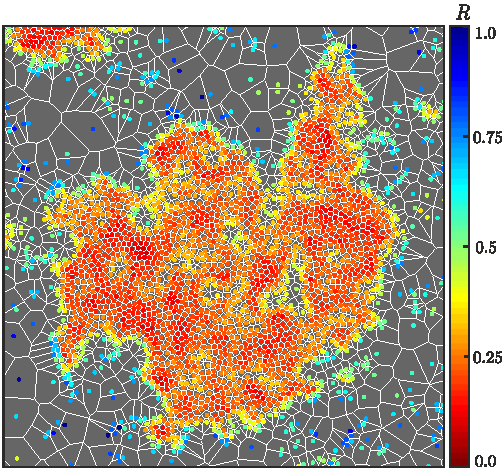
\includegraphics[width=0.7\textwidth]{MPI-Figure1}
\caption{Пример конденсированного кластера в системе с потенциалом Леннарда-Джонса. Ячейки вороного раскрашены в белый цвет, частицы раскрашены по величине параметра $R$.}
\label{risIrreg}
\end{center}
\end{figure}

На рисунке \ref{risIrreg} представлен конденсированный кластер, частицы которого раскрашены в соответствии с параметром иррегулярности. Чем он меньше, чем более упорядочена система. В идеальном кристалле данный параметр равен нулю.

Поскольку параметр $R$ мал для частиц принадлежащих кластерам конденсата, мы можем использовать следующее неравенство для их определения:

\begin{equation}
R < R_t,
\end{equation}

где $R_t$ - порог для частиц конденсата.

\begin{figure}[h]
\begin{center}
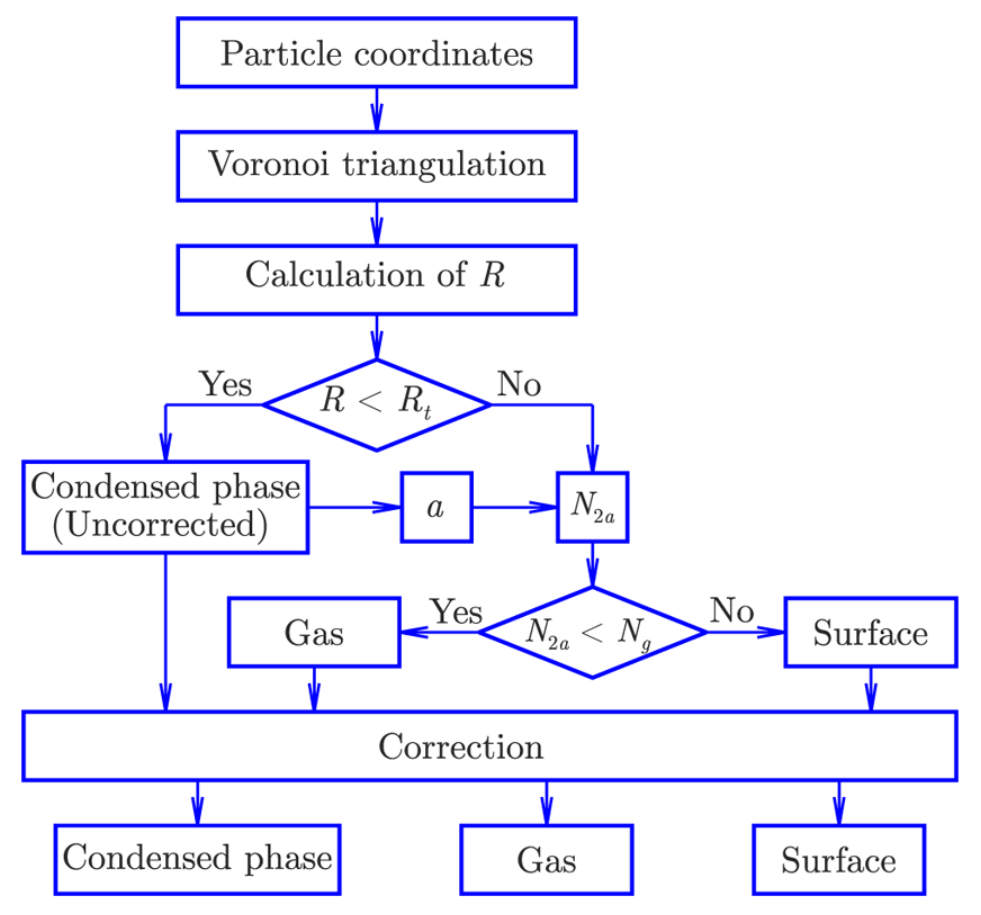
\includegraphics[width=0.5\textwidth]{shem_class}
\caption{Полная схема классификации частиц в системе.}
\label{risShemClass}
\end{center}
\end{figure}

Полная схема классификации частиц в системе, которая использует только координаты, представлена на рисунке \ref{risShemClass},
где $a$ - среднее расстояние между частицами; $N_g$ - некоторое пороговое значение для газовых частиц, находящихся на расстоянии $2a$ от выбранной частицы; $N_{2a}$ - число частиц, находящихся на расстоянии менее $2a$ от выбранной частицы. Если выполняется условие $N_{2a} < N_{g}$, то частица распознается как газ.
В данной работе константы приняты равными $R = 0.5, N_g = 5$.


По причине больший флуктуаций величины $R$, кроме обрезки по параметру $R_t$, требуется корректировка фаз.


Корректировка фаз включает в себя следующие условия:
\begin{itemize}
\item частица конденсата, не имеющая среди своих соседей частиц того же типа, является поверхностью.
\item частица конденсата, которая имеет среди соседних частиц, газовую частицу, является поверхностью.
\item газовая частица, не имеющая соседних частиц того же класса,  является поверхностью.
\item частица поверхности, все соседи которой принадлежат к классу "конденсат" или "газ", так же принадлежат к этому классу.
\end{itemize}
Данная корректировка повторяется несколько раз. Было установлено, что пяти раз достаточно, для приемлемого результата классификации.

\begin{figure}[h]
\begin{center}
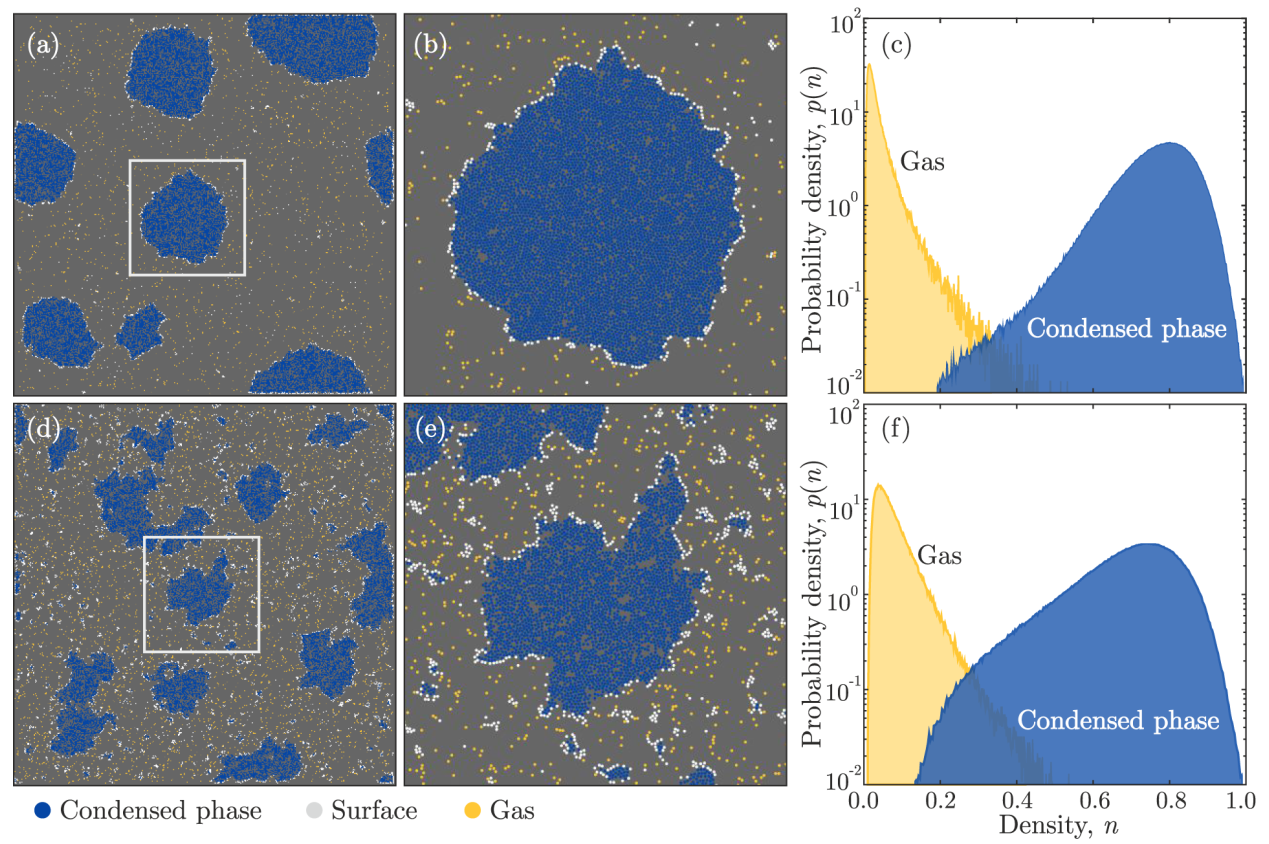
\includegraphics[width=0.8\textwidth]{articlePhaseAndDensity}
\caption{Слева - результат работы алгоритма, представленного на рисунке \ref{risShemClass}. Частицы разделены на 3 класса различными цветами: конденсат - синий, поверхность - белый, газ - желтый. Справа - плотность вероятности нахождения частицы газа и конденсата с данной плотностью.}
\label{risClassification}
\end{center}
\end{figure}

На рисунке \ref{risClassification} представлен результат классификации частиц в системе данным методом. Однако у данного алгоритма есть ряд недостатков. Так например возможны случаи распознавания пустот с газом внутри конденсированного кластера, как его часть, а также наблюдаются крупные скопления частиц поверхности, внутри который нет частиц, распознанных как конденсат.


После классификации всех частиц в системе и расчета плотностей по формуле \ref{eqRho}, возможно рассчитать мат. ожидание плотности конденсированных частиц и газа отдельно.
Рассчитав таким образом плотности при различных температурах, можно построить фазовую диаграмму в координатах $\rho, T$.


Однако прямой расчет плотности корректно работает только для конденсированных частиц, так как флуктуации размеров ячеек не велики, и на их размер не оказывают влияния частицы газа и поверхности. На площадь газовых частиц существенный эффект оказывают частицы поверхности, которые занимают сопоставимый объем, существенно увеличивая плотность первых.


В рамках данной работы был существенно переработан алгоритм корректировки фаз, который помимо условий представленных в оригинальной работе включает дополнительные условия:
\begin{itemize}
\item частица поверхности, не имеющая среди соседей частиц газа, является конденсатом.
\item поверхностная частица, не имеющая среди соседей частиц конденсата, является газом.

\item частицы конденсата, плотность которых сопоставима с плотностью поверхностных частиц, являются поверхностью. Данная проверка делается дважды (перед всеми остальными и после).

\item частица конденсата, которая имеет меньше 3 соседних частиц, так же принадлежащих к конденсату, является поверхностью.
\end{itemize}


Данные условия позволяют отделить крупные пустоты внутри кристалла от самого кристалла, и определить крупные скопления поверхностных частиц как небольшие кластеры конденсата или газ.


Так же был переработан алгоритм вычисления плотности газа в системе. Она вычисляется косвенно, по формуле:

\begin{equation}
\rho_{gas} = \frac{N_{g}}{S - (N_{b} + N_{c}) / \mathbb{M}\rho_c},
\label{eqGas}
\end{equation}

где $S$ - полная площадь; $N_g, N_b, N_c$ - число частиц газа, поверхности и конденсата соответственно; $\mathbb{M}\rho_c$ - мат. ожидание плотности частиц конденсата.

При данном подходе площадь поверхностных частиц считается равной плотности конденсата, что позволяет более объективно вычислять плотность газа.


\section{Построение фазовых диаграмм для различных потенциалов взаимодействия}\label{C2_2}

В данной работе для изучения влияния дальнодействия притяжения на фазовые диаграммы, были выбраны системы с потенциалом взаимодействия обобщенного Леннарда - Джонса (уравнение \ref{eqLJ}), с изменяющейся степенью слагаемого, отвечающего за притяжение.

\begin{equation}
U(r) = 4\varepsilon \left[ \left(\frac{\sigma}{r}\right)^{12} - \left(\frac{\sigma}{r}\right)^{m} \right]
\label{eqLJ}
\end{equation}

Моделирование данных систем было было проведено в программе LAMMPS, с параметрами, указанными в таблице \ref{tablParam}, где $m$ - степень в уравнении \ref{eqLJ}; $\Delta T$ - шаг по температуре;  $\rho$ - плотность системы. Во всех численных экспериментах рассматривалась система в $NVT$ ансамбле, состоящая из 3600 частиц. В ходе моделирования было проделано 600000 итераций изменения системы, между которыми было $0.05\tau$ времени, где $\tau$ - безразмерное эффективное время, обезразмеренное на константы системы. В процессе моделирования данные выводились с периодом в 100 итераций расчета системы, всего таким образом было получено 6000 состояний системы с интервалом в $0.5\tau$ по времени. Что бы исключить эффекты, связанные с релаксацией системы, во всех моделированиях были взяты только последние 150 состояний, в которых система уже отрелаксировала.   

Все величины, встречающиеся в данной работе далее, являются обезразмеренными на константы моделирования, такие как масса частиц, постоянную Больцмана, $\varepsilon$ и $\sigma$ в уравнении \ref{eqLJ} потенциала , равные единице.


\begin{table}[h]
\begin{center}
\begin{tabular}{| l | l | l | l | l |}
\hline
    & LJ12-3 & LJ12-4 & LJ12-5 & LJ12-6 \\ \hline
$m$   &    3    &     4   &    5    &    6    \\ \hline
$\Delta T$ & 0.03 & 0.03 & 0.02 & 0.02 \\ \hline
$\rho$ & 0.28  &  0.4  &  0.4  &  0.4  \\ \hline
$\Delta t$ & 0.5 & 0.5 & 0.5 & 0.5 \\ \hline
\end{tabular}
\end{center}
\caption{Параметры моделирования исследуемых систем. $m$ - степень слагаемого в уравнении \ref{eqLJ}; $\Delta T$ - шаг по температуре;  $\rho$ - плотность системы; $\Delta t$ - шаг по времени между кадрами.}
\label{tablParam}
\end{table}

На примере потенциала Леннарда - Джонса продемонстрированна работа модифицированного алгоритма распознавания фаз при различной температуре. На рисунке \ref{risvoronoiExp} изображено разбиение системы на ячейки Вороного, затем проводится расчет параметра иррегулярности, представленного на рисунке \ref{risIregExp}, затем, после корректировки фаз, мы получаем принадлежность каждой частицы к классу конденсата, газа или поверхности (рисунок \ref{risClassExp}).


\begin{figure}[h]
\begin{center}
\includegraphics[width=0.7\textwidth]{Voronoi}
\caption{Разбиение на ячейки Вороного исследуемой системы на примере системы c потенциалом взаимодействия Леннарда-Джонса при различной температуре.}
\label{risvoronoiExp}
\end{center}
\end{figure}



\begin{figure}[h]
\begin{center}
\includegraphics[width=0.7\textwidth]{RG}
\caption{Параметр иррегулярности $R$ в исследуемой системе, на примере потенциала взаимодействия Леннарда-Джонса при различной температуре.}
\label{risIregExp}
\end{center}
\end{figure}



\begin{figure}[h]
\begin{center}
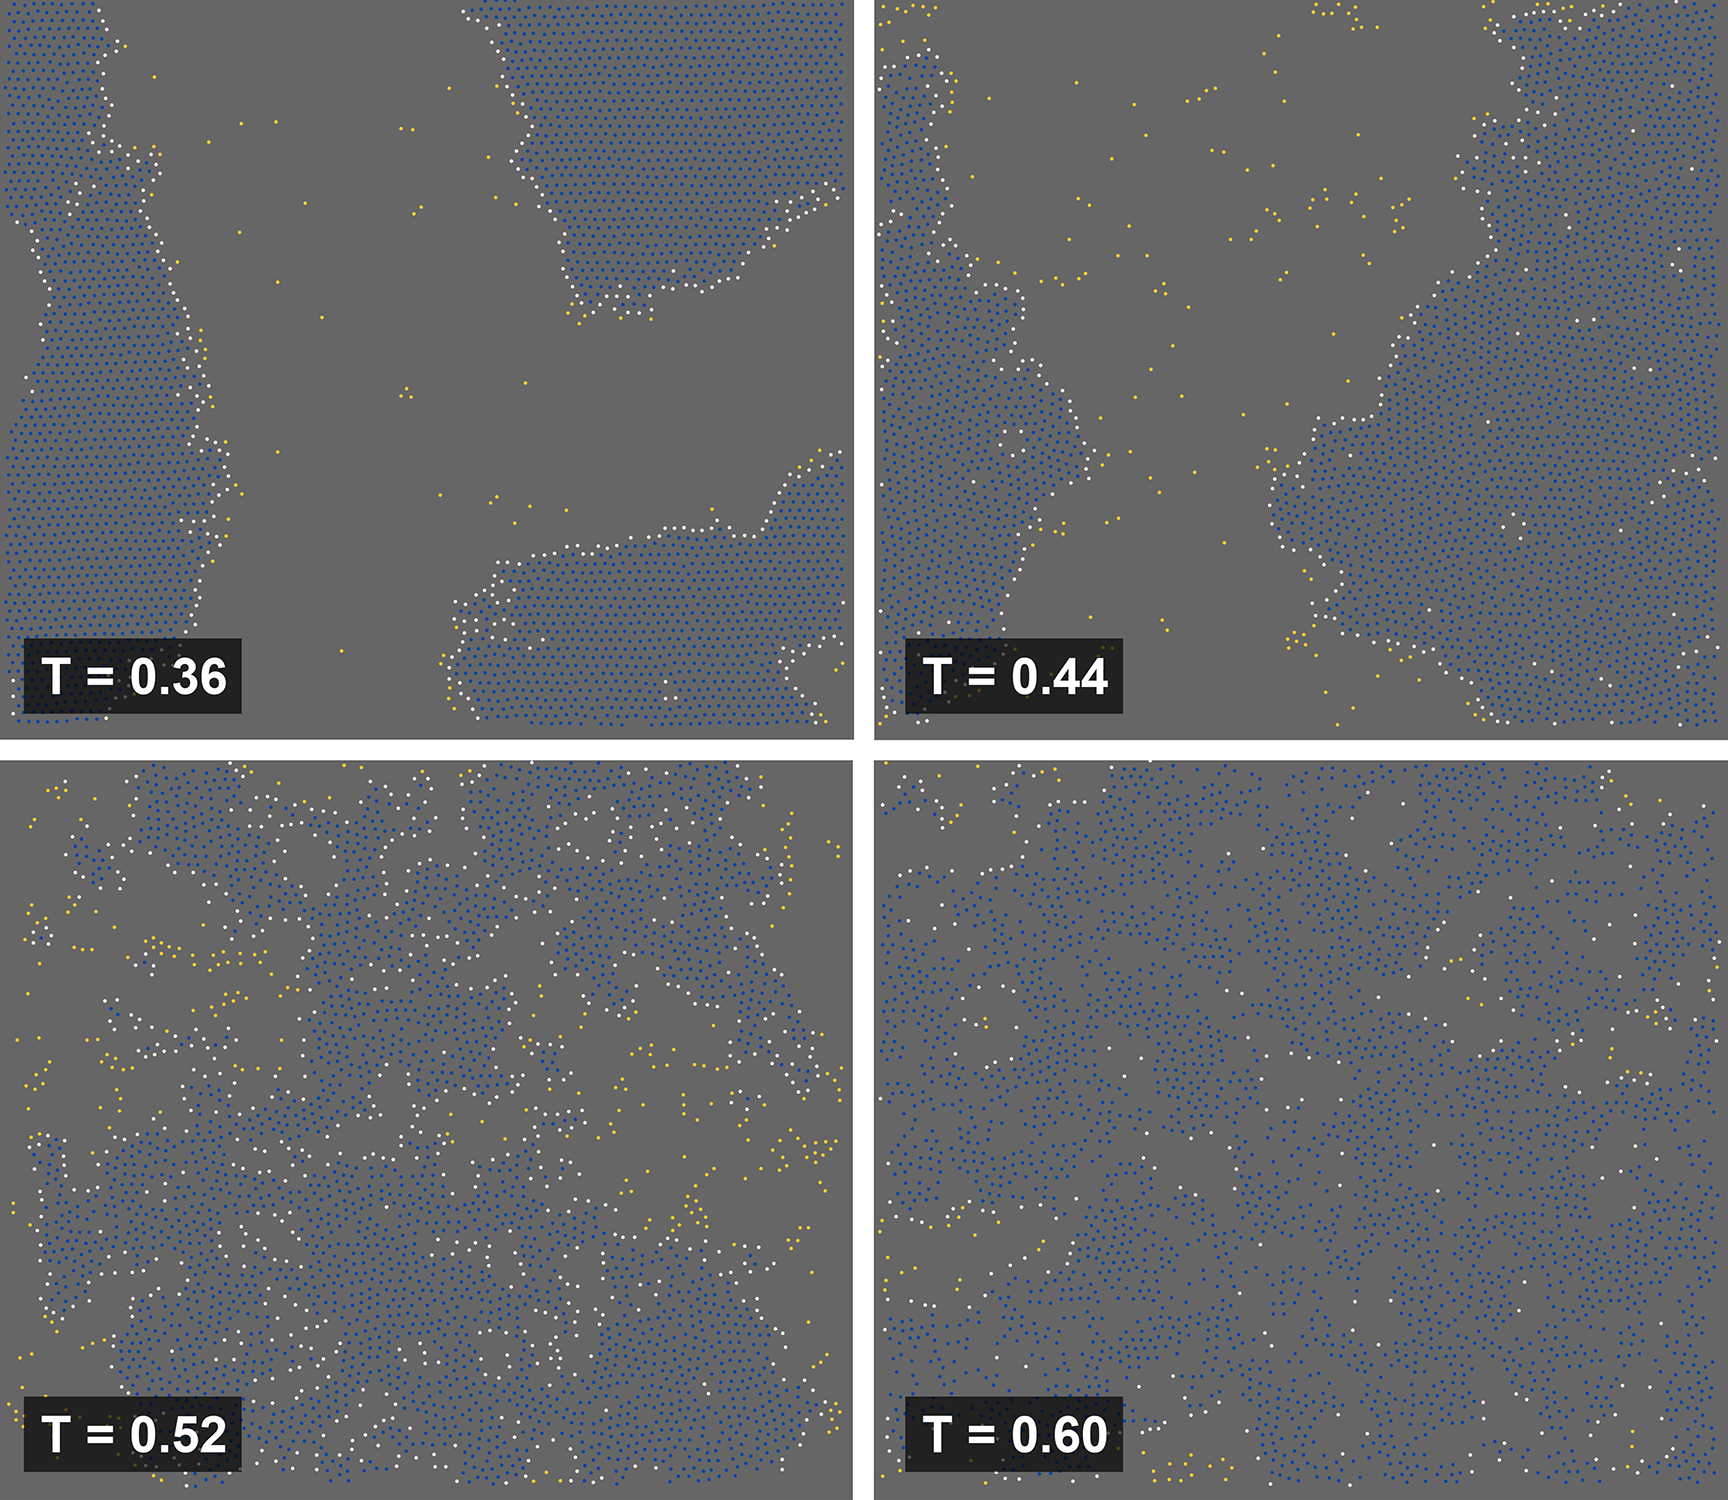
\includegraphics[width=0.7\textwidth]{classification}
\caption{Классификация частиц в исследуемой системы на примере системы c потенциалом взаимодействия Леннарда-Джонса при различной температуре.}
\label{risClassExp}
\end{center}
\end{figure}

Как можно увидеть на рисунке \ref{risClassExp}, данный метод лишен недостатков, описанных в главе \ref{C2_1}, связанных с распознаванием фаз.




\begin{figure}[h]
\begin{center}

\begin{minipage}[h]{0.45\linewidth}
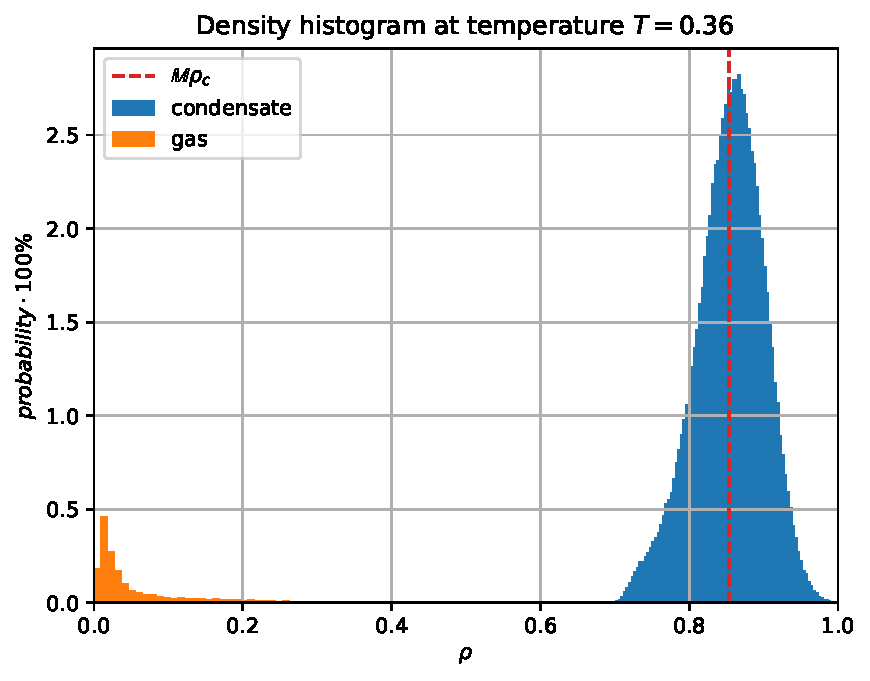
\includegraphics[width=\textwidth, keepaspectratio]{plot_hist_all_0.360}
\end{minipage}
%\hfill
\begin{minipage}[h]{0.45\linewidth}
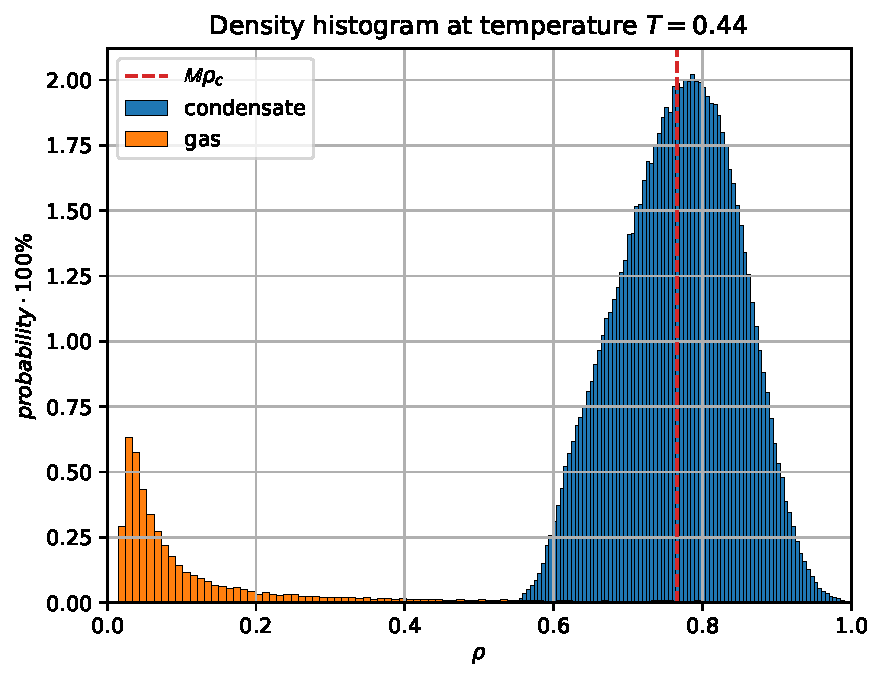
\includegraphics[width=\textwidth, keepaspectratio]{plot_hist_all_0.440}
\end{minipage}

%\vfill

\begin{minipage}[h]{0.45\linewidth}
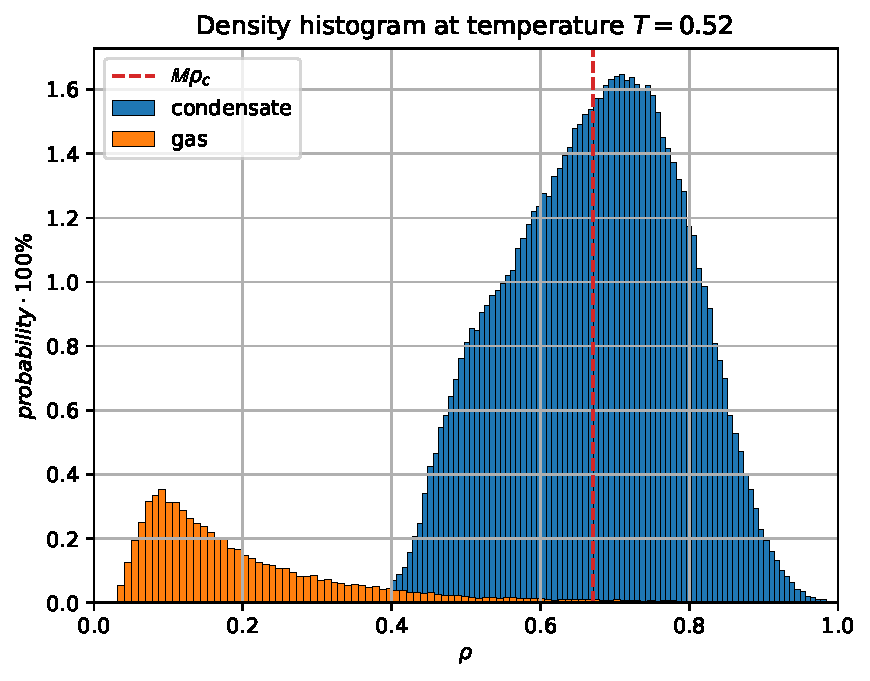
\includegraphics[width=\textwidth, keepaspectratio]{plot_hist_all_0.520}
\end{minipage}
%\hfill
\begin{minipage}[h]{0.45\linewidth}
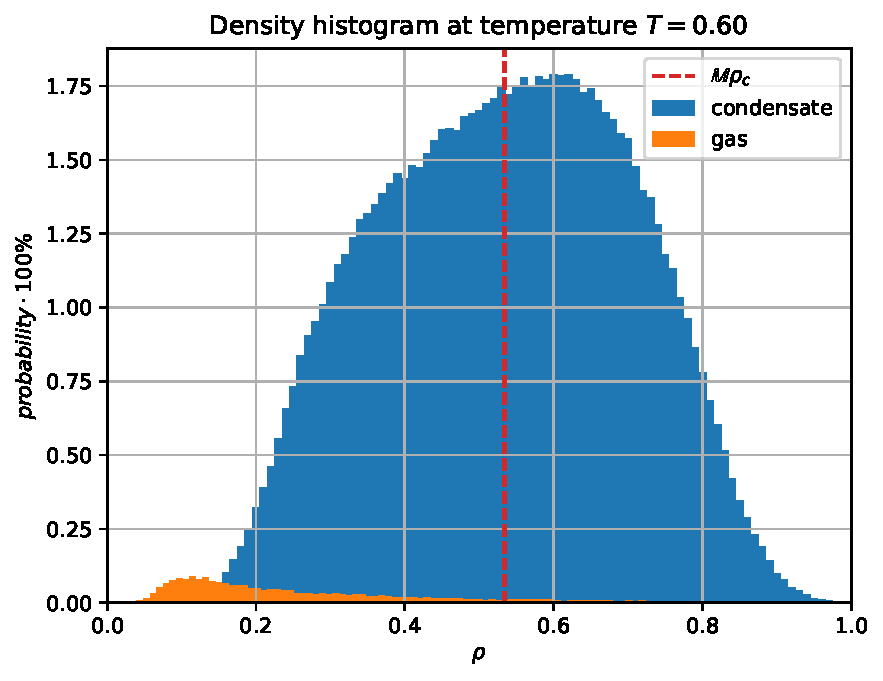
\includegraphics[width=\textwidth, keepaspectratio]{plot_hist_all_0.600}
\end{minipage}
\caption{Распределение плотностей частиц конденсата и газа при различных температурах. Синим цветом обозначен конденсат, оранжевым  - газ.}
\label{risRhoM}
\end{center}
\end{figure}


После классификации частиц, можно приступать к определению мат. ожидания плотности газа и конденсата. На рисунке \ref{risRhoM} изображена график вероятности найти частицу в данной фазе с данной плотностью. Через значение плотности конденсата, указанное на рисунке красной пунктирной линией, можно по формуле \ref{eqGas} найти плотность газа в системе, и повторяя данную процедуру при различной температуре и значениям степени $m$, получаем фазовые диаграммы для систем с различными потенциалами взаимодействия, изображенные на рисунке \ref{risPhaseDiagrammExp}.


\begin{figure}[h]
\begin{center}
\begin{minipage}[h]{0.45\linewidth}
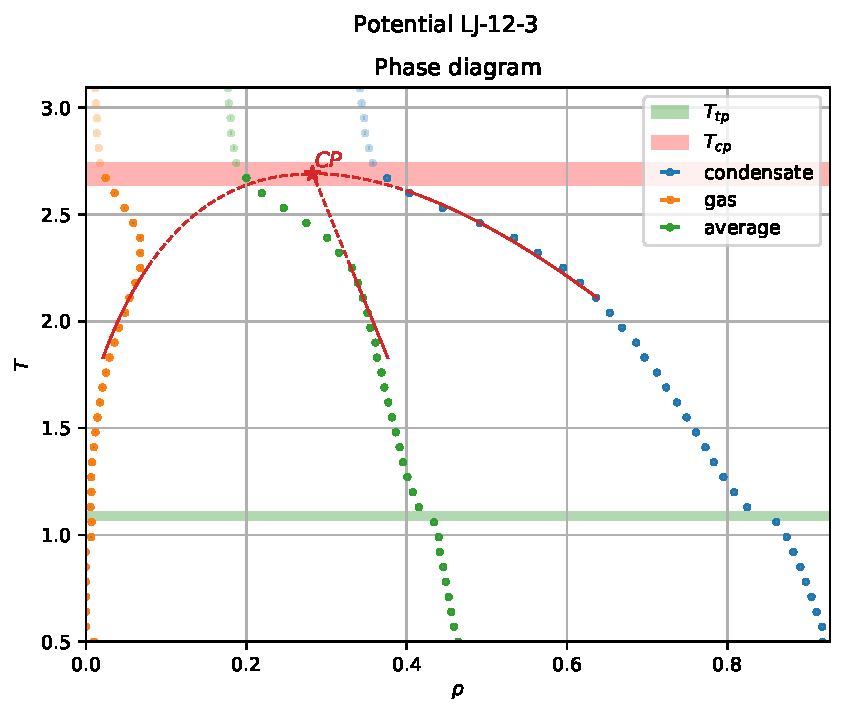
\includegraphics[width=\textwidth, keepaspectratio]{plot_phase_diagram_Potential LJ-12-3_1}
\end{minipage}
%\hfill
\begin{minipage}[h]{0.45\linewidth}
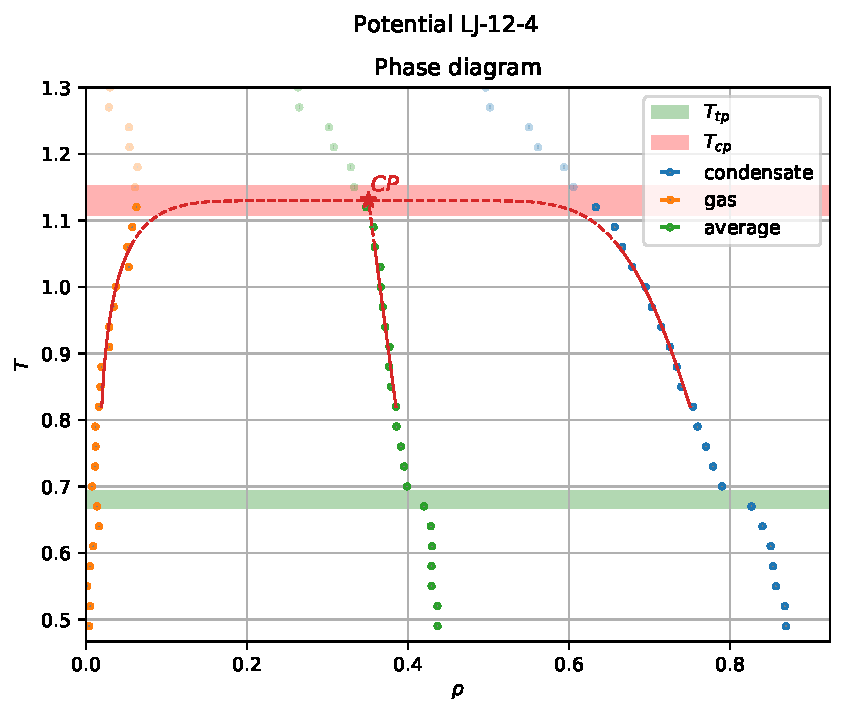
\includegraphics[width=\textwidth, keepaspectratio]{plot_phase_diagram_Potential LJ-12-4_1}
\end{minipage}


\begin{minipage}[h]{0.45\linewidth}
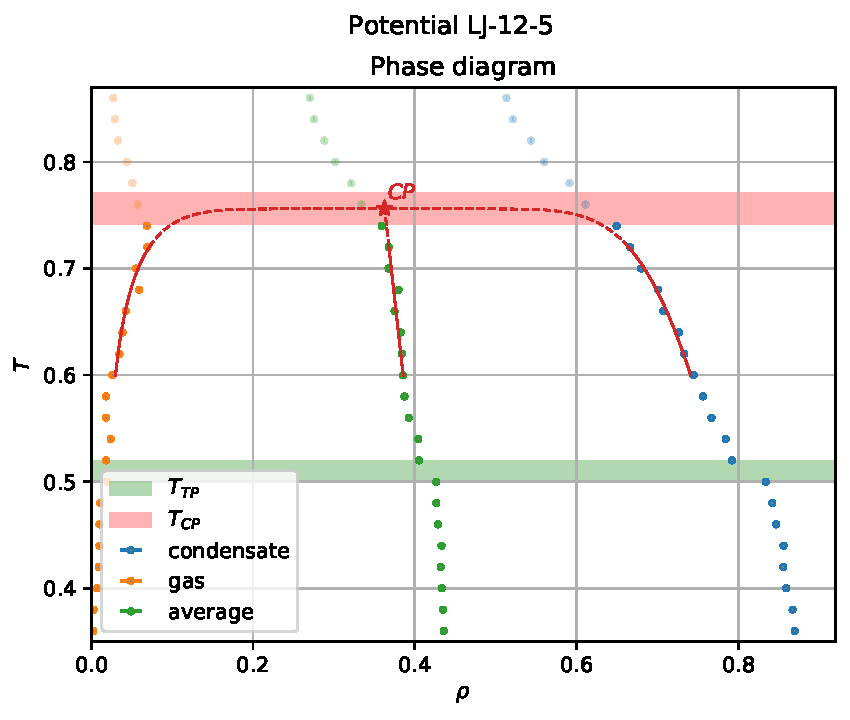
\includegraphics[width=\textwidth, keepaspectratio]{plot_phase_diagram_Potential LJ-12-5_1}
\end{minipage}
%\hfill
\begin{minipage}[h]{0.45\linewidth}
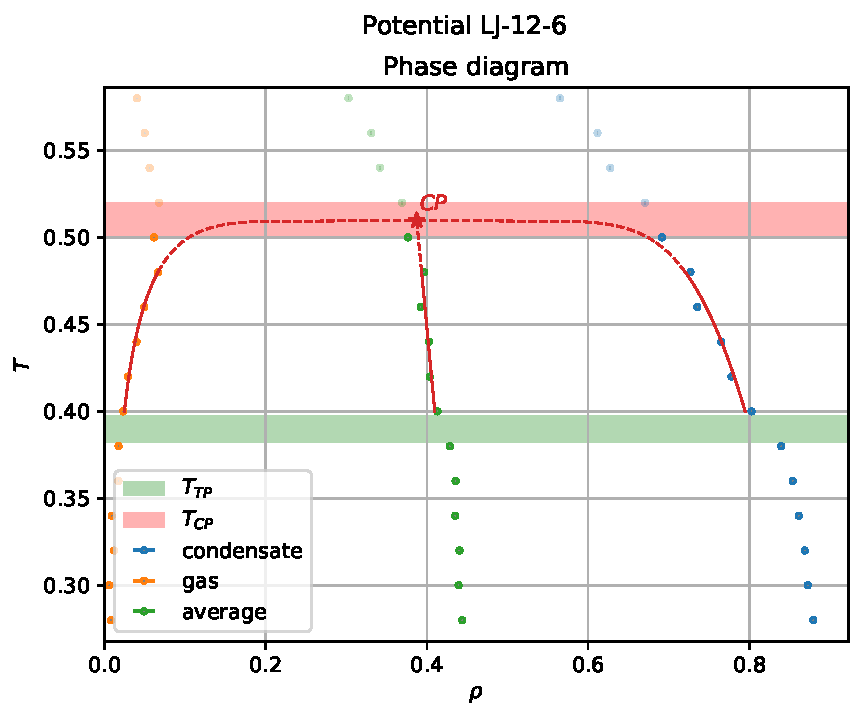
\includegraphics[width=\textwidth, keepaspectratio]{plot_phase_diagram_Potential LJ-12-6_1}
\end{minipage}
\caption{Фазовые диаграммы для систем с различными потенциалами взаимодействия. Подробности в основном тесте.}
\label{risPhaseDiagrammExp}
\end{center}
\end{figure}


Как известно из теории \cite{fitPhase}, фазовые диаграммы в координатах $\rho, T$, вблизи критики описываются следующими уравнениями: 

\begin{equation}
\begin{aligned}
\rho_l - \rho_g &\simeq A (T_{CP} - T)^{\beta_c} \\
\frac{\rho_l + \rho_g}{2} &\simeq \rho_{CP} + a(T_{CP} - T)
\end{aligned}
\label{eqFitFhase}
\end{equation}

где $T_{CP}, \rho_{CP}$ - эффективная температура и плотность критической точки; $A, a$ - варьируемые параметры; $\rho_l, \rho_g$ - плотность жидкости и газа соответственно; $\beta_c$ - критический индекс.

Согласно источнику \cite{classCrit}, класс универсальности системы зависит от диапазона притяжения. Так, система LJ12-3 демонстрирует классическое поведение, для которого $\beta_c = 1/2$, для всех остальных потенциалов, рассматриваемых в данной работе этот параметр равен 1/8.

Для более удобного определения критической точки с помощью аппроксимации бинодалей можно записать систему уравнений \ref{eqFitFhase} в следующем виде:
\begin{equation}
f_g(T) = \frac{T-a}{b} - A(T_{CP} - T)^{\beta_c}
\label{eqFitFhaseGas}
\end{equation}
\begin{equation}
f_l(T) = \frac{T-a}{b} + A(T_{CP} - T)^{\beta_c}
\label{eqFitFhaseLicuid}
\end{equation}
\begin{equation}
f_a(T) = \frac{T-a}{b},
\label{eqFitFhaseAverage}
\end{equation}

где уравнение \ref{eqFitFhaseGas} описывает газовую бинодаль, \ref{eqFitFhaseLicuid} - конденсированную, \ref{eqFitFhaseAverage} - их среднее значение; $A, a, b, T_{CP}$ - варьируемые параметры. 


Тогда можно составить функцию невязки, при минимизации которой получить наилучшую аппроксимацию бинодалей и значение критической температуры и плотности.

Условие наилучшей подгонки выглядит следующим образом:
\begin{equation}
\min \left(\sum\limits_{k} \left[ f_g(T_{g, k}) - n_{g, k}  \right]^2 + \sum\limits_{k} \left[ f_l(T_{l, k}) - n_{l, k}  \right]^2 + \sum\limits_{k} \left[ f_a(T_{g, k}) - n_{a, k}  \right]^2 \right),
\label{eqFitResidual}
\end{equation}
где суммирование производится по выбранным для аппроксимации точкам, а $n_g, n_l, n_a$ - соответствующие плотности выбранных точек. 

Точки могут быть выбраны не обязательно из одного температурного диапазона, для лучшей точности чаще всего, выбирается немного различный диапазон. Это связано с некоторыми особенностями данного метода. Например вблизи критики, из-за выравнивания плотности, существенно падает среднее значение параметра иррегулярности, из-за чего большинство частиц в системе начинает распознаваться как газ. В связи с этим резко начинает падать плотность газа, что не соответствует действительности, поэтому газовая бинодаль аппроксимируется только до момента, пока не меняет знака вторая производная плотности по температуре. Данный эффект также влияет и на среднее значение газовой и конденсированной бинодали, поэтому среднее значение также аппроксимируется только до данной температуры. Конденсированная ведет себя более стабильно, и аппроксимация может проводиться по температурам чуть больше, чем для газа и среднего значения.

Аппроксимация, проведенная данным методом, изображена на рисунке \ref{risPhaseDiagrammExp}, где красной цельной линией обозначены точки, участвовавшие в аппроксимации, а красной штриховой - экстраполяция функций \ref{eqFitFhaseGas}, \ref{eqFitFhaseLicuid}, \ref{eqFitFhaseAverage} c найденными на предыдущем шаге константами.

Как можно видеть она довольно хорошо аппроксимирует точки на бинодалях, что позволяет довольно точно определить критическую температуру и критическую плотность системы.

Параметры системы, определенные данным способом приведены в таблице \ref{tablSystemConst}.

\begin{table}[h]
\begin{center}
\begin{tabular}{| l | l | l | l | l |}
\hline
    & LJ12-3 & LJ12-4 & LJ12-5 & LJ12-6         \\ \hline
$T_{CP}$    & 2.69  &  1.13   &  0.76  &    0.51   \\ \hline
$T_{TP}$    & 1.09  & 0.68    & 0.51   & 0.40   \\ \hline
$\rho_{CP}$ & 0.28  &  0.35   &  0.36   &  0.39   \\ \hline
\end{tabular}
\end{center}
\caption{Параметры фазовой диаграммы для различных потенциалов.}
\label{tablSystemConst}
\end{table}

Зная критические точки для потенциалов с различным притяжением, можно установить роль притяжения потенциала в фазовой диаграмме вещества. На рисунке \ref{risTcpTtp} изображена зависимость отношения температур критической точки к тройной от степени слагаемого в потенциале \ref{eqLJ} отвечающего за притяжение. 


\begin{figure}[h]
\begin{center}
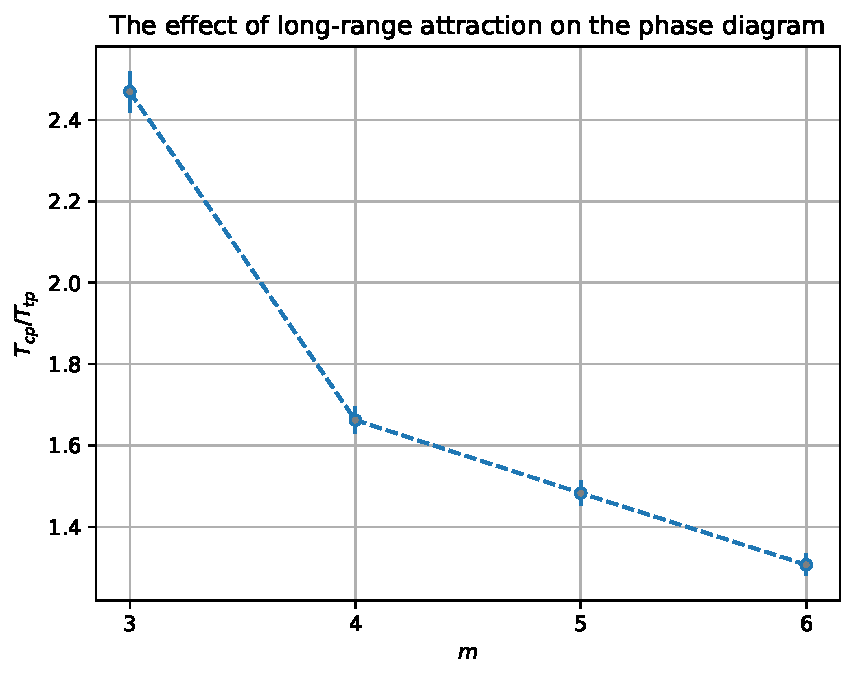
\includegraphics[width=0.7\textwidth]{effect of long-range attraction}
\caption{Отношение температур критической к тройной в зависимости от степени $m$ слагаемого в потенциале, отвечающего за притяжение.}
\label{risTcpTtp}
\end{center}
\end{figure}

По этим данным можно утверждать, что, скорей всего, функция изображенная на \ref{risTcpTtp}, линейна для систем, относящихся к одному классу универсальности.


\section{Анализ гистограмм распределения}\label{C2_3}

Из теории следует \cite{Landau}, что равновесные колебания вблизи среднего значения определяются по уравнению состояния системы, и соответствующая функция распределения вероятности $p(V)$ равна:
\begin{equation}
p(V) \varpropto exp \left[ \frac{1}{2T} \left( \frac{\partial P}{\partial V} \right)  \left(V - V_0 \right)^2 \right],
\label{eqPv}
\end{equation}
где $P$ - давления; $V_0$ - максимум распределения объема частиц; $V$ - объем (площадь в $2D$ случае) частиц.
Тогда мы можем численно оценить производную $\frac{\partial P}{\partial V}$ и термодинамические величины с ней связанные.

Перепишем формулу \ref{eqPv} для колебаний плотности системы сделав замену $V = 1 / \rho$, и получим следующее уравнение:
\begin{equation}
\begin{aligned}
p(\rho) &\varpropto exp \left[ - K \left(\rho_{max}- \rho \right)^2 \right] \\
K &= \frac{1}{2T\rho_{max}^2} \left( \frac{\partial P}{\partial \rho} \right)
\end{aligned}
\label{eqFitRho}
\end{equation}
где $\rho_{max}$ - плотность максимума распределения.


\begin{figure}[htbp!]
\begin{center}
\begin{minipage}[h]{0.45\linewidth}
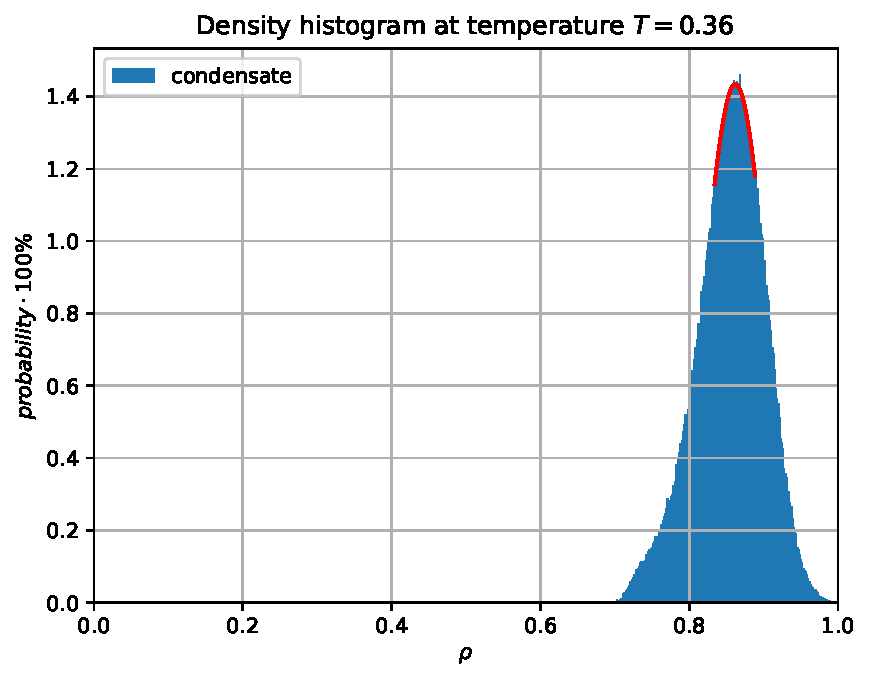
\includegraphics[width=\textwidth, keepaspectratio]{plot_hist_fit_0.360}
\end{minipage}
%\hfill
\begin{minipage}[h]{0.45\linewidth}
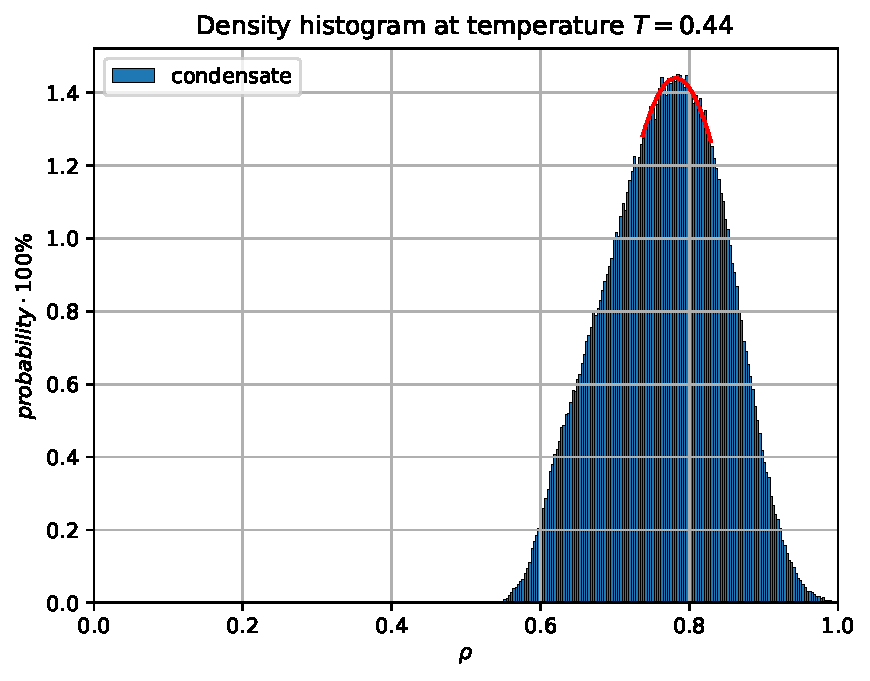
\includegraphics[width=\textwidth, keepaspectratio]{plot_hist_fit_0.440}
\end{minipage}

\begin{minipage}[h]{0.45\linewidth}
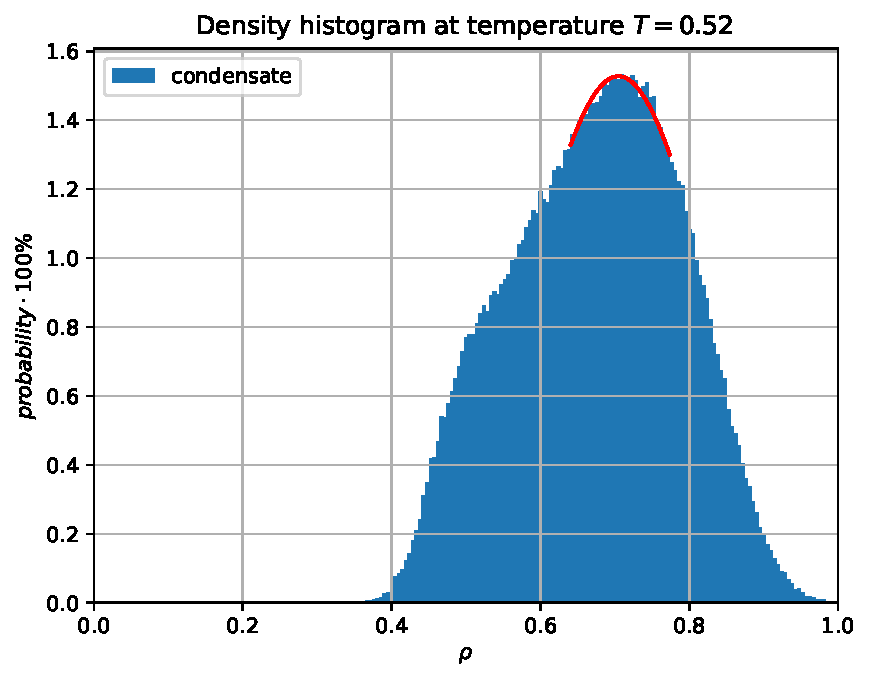
\includegraphics[width=\textwidth, keepaspectratio]{plot_hist_fit_0.520}
\end{minipage}
%\hfill
\begin{minipage}[h]{0.45\linewidth}
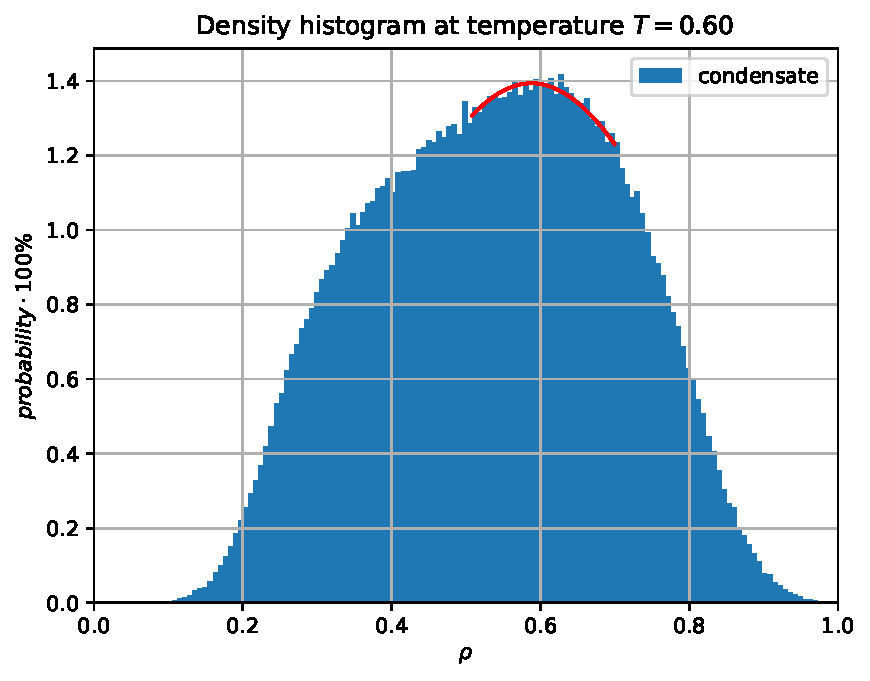
\includegraphics[width=\textwidth, keepaspectratio]{plot_hist_fit_0.600}
\end{minipage}
\caption{Аппроксимация пика распределения при различной температуре.}
\label{risHistFit}
\end{center}
\end{figure}

Аппроксимируя данным уравнением верхушку распределения плотностей для различных температур каждой системы (рисунок \ref{risHistFit}), получаем температурную зависимость коэффициента $K$ представленную на рисунке \ref{risK}.

\begin{figure}[htbp!]
\begin{center}
\begin{minipage}[h]{0.45\linewidth}
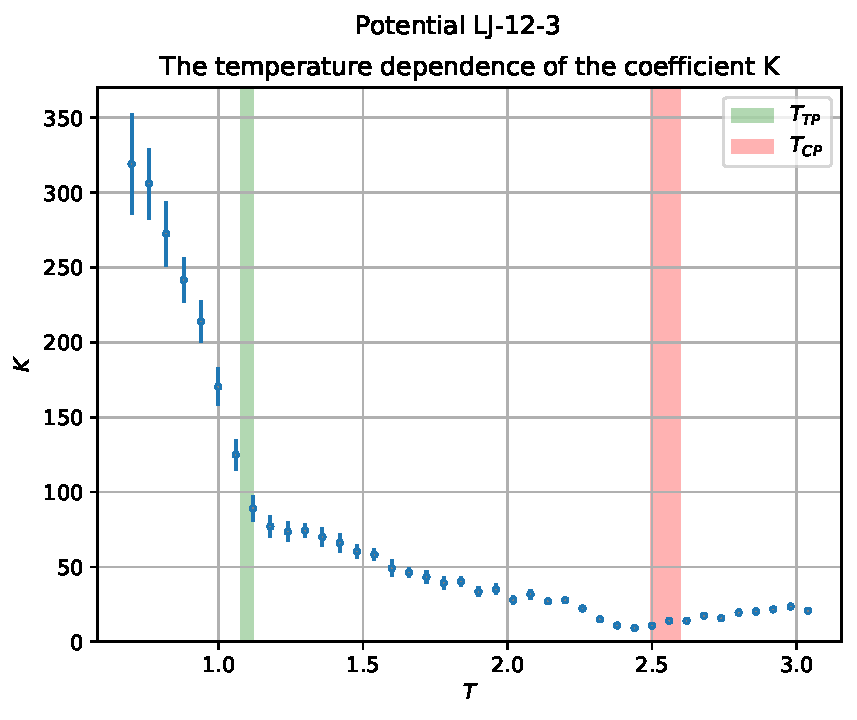
\includegraphics[width=\textwidth, keepaspectratio]{plot_K_Potential LJ-12-3_1}
\end{minipage}
%\hfill
\begin{minipage}[h]{0.45\linewidth}
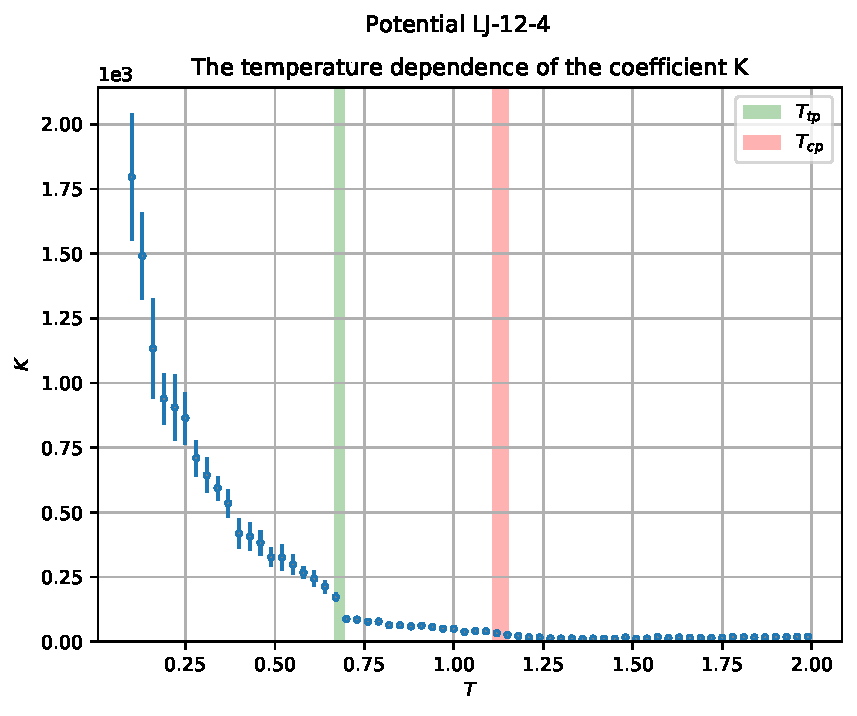
\includegraphics[width=\textwidth, keepaspectratio]{plot_K_Potential LJ-12-4_1}
\end{minipage}

%\vfill

\begin{minipage}[h]{0.45\linewidth}
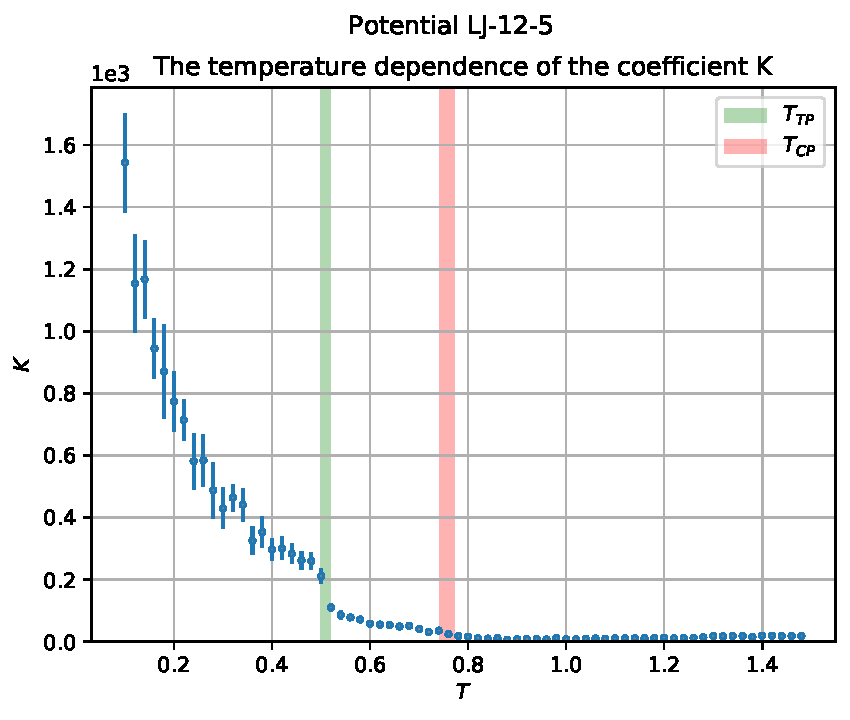
\includegraphics[width=\textwidth, keepaspectratio]{plot_K_Potential LJ-12-5_1}
\end{minipage}
%\hfill
\begin{minipage}[h]{0.45\linewidth}
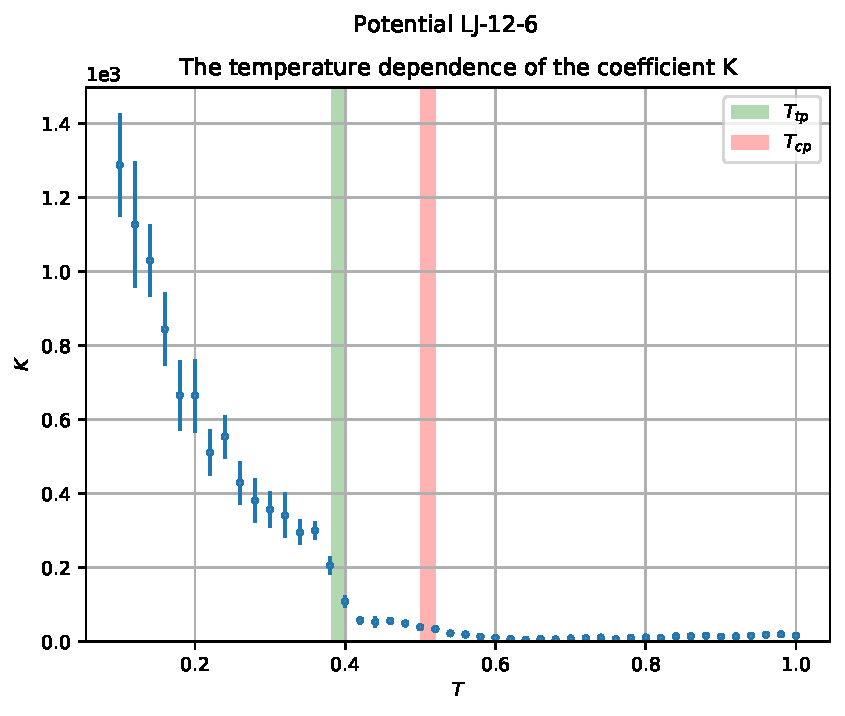
\includegraphics[width=\textwidth, keepaspectratio]{plot_K_Potential LJ-12-6_1}
\end{minipage}
\caption{Температурная зависимость коэффициента $K$.}
\label{risK}
\end{center}
\end{figure}

Текст


\begin{figure}[htbp!]
\begin{center}
\begin{minipage}[h]{0.45\linewidth}
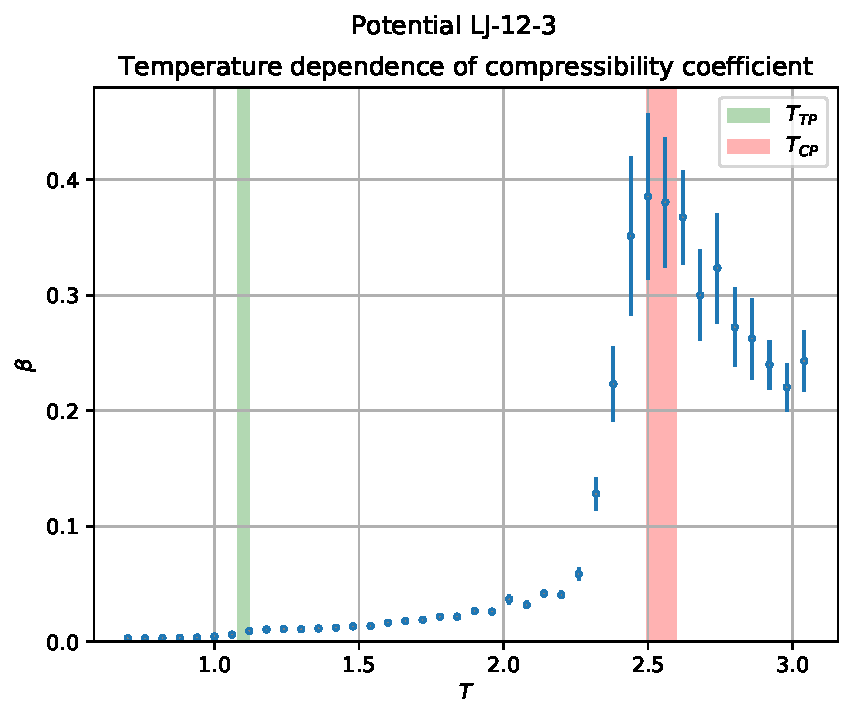
\includegraphics[width=\textwidth, keepaspectratio]{plot_compress_Potential LJ-12-3_1}
\end{minipage}
%\hfill
\begin{minipage}[h]{0.45\linewidth}
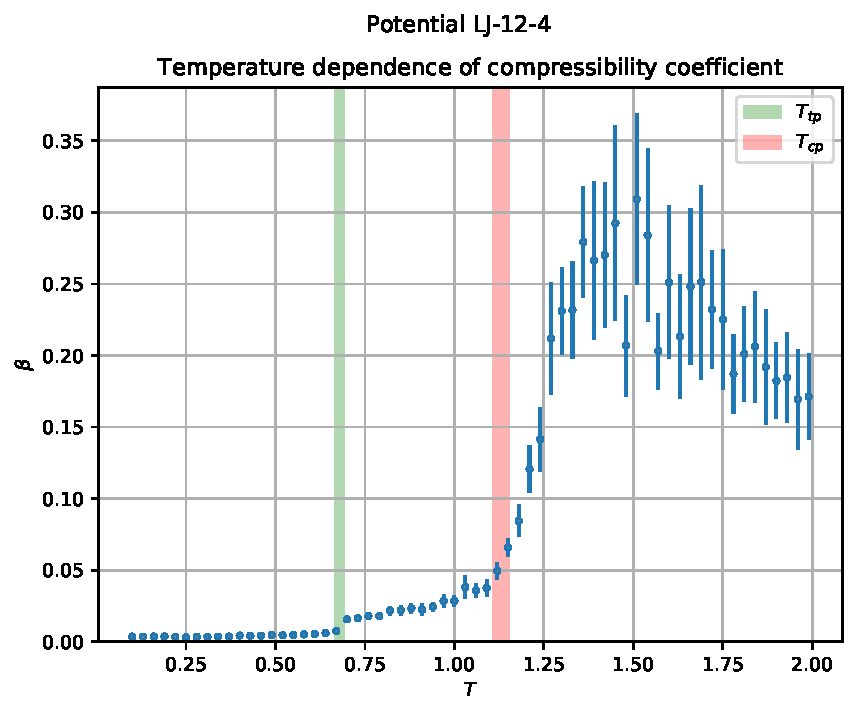
\includegraphics[width=\textwidth, keepaspectratio]{plot_compress_Potential LJ-12-4_1}
\end{minipage}

%\vfill

\begin{minipage}[h]{0.45\linewidth}
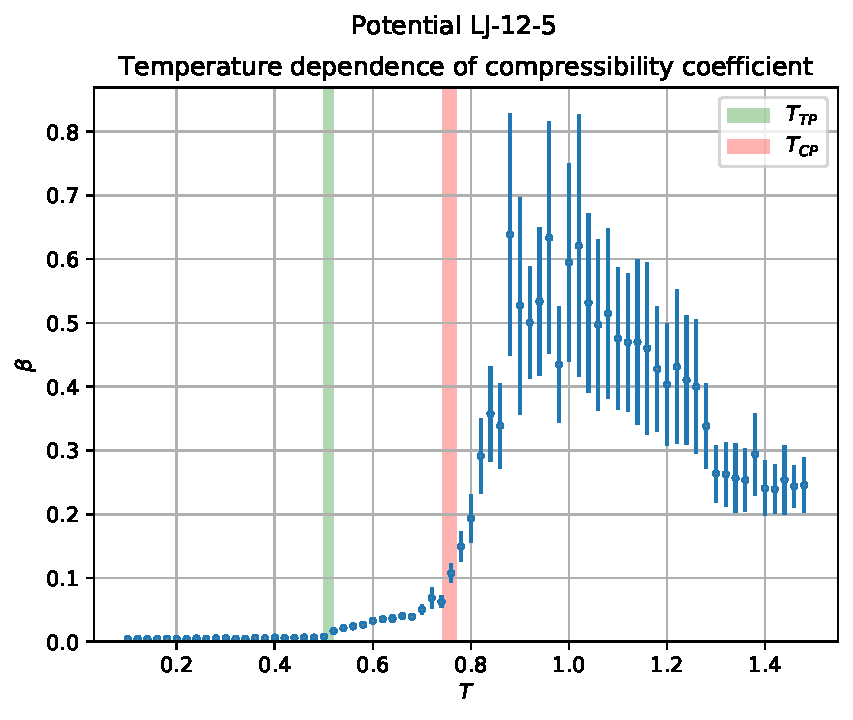
\includegraphics[width=\textwidth, keepaspectratio]{plot_compress_Potential LJ-12-5_1}
\end{minipage}
%\hfill
\begin{minipage}[h]{0.45\linewidth}
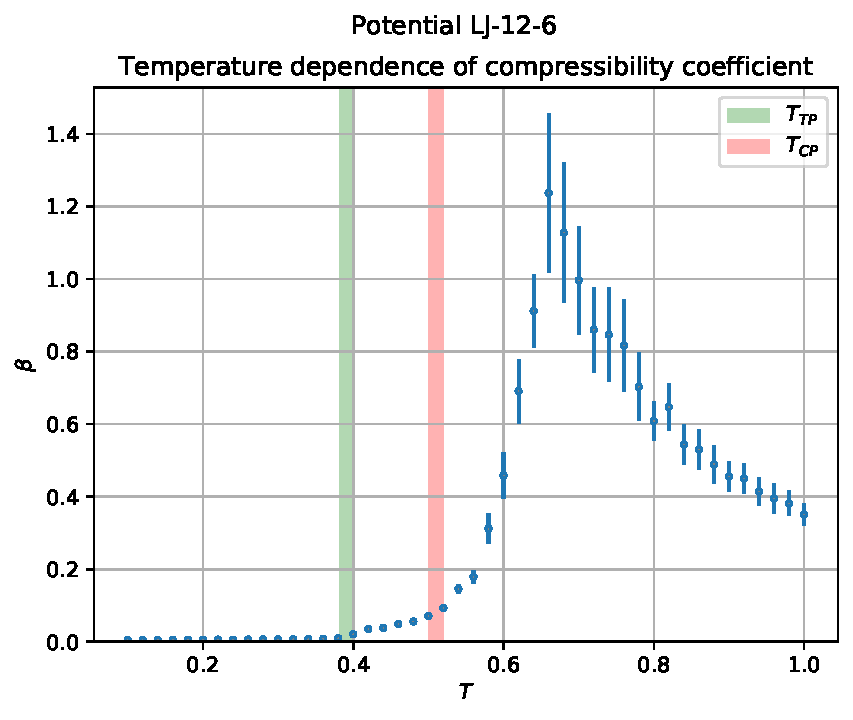
\includegraphics[width=\textwidth, keepaspectratio]{plot_compress_Potential LJ-12-6_1}
\end{minipage}
\caption{Температурная зависимость коэффициента $\beta$ сжимаемости вещества.}
\label{ris13}
\end{center}
\end{figure}

Текст

\begin{figure}[htbp!]
\begin{center}
\begin{minipage}[h]{0.45\linewidth}
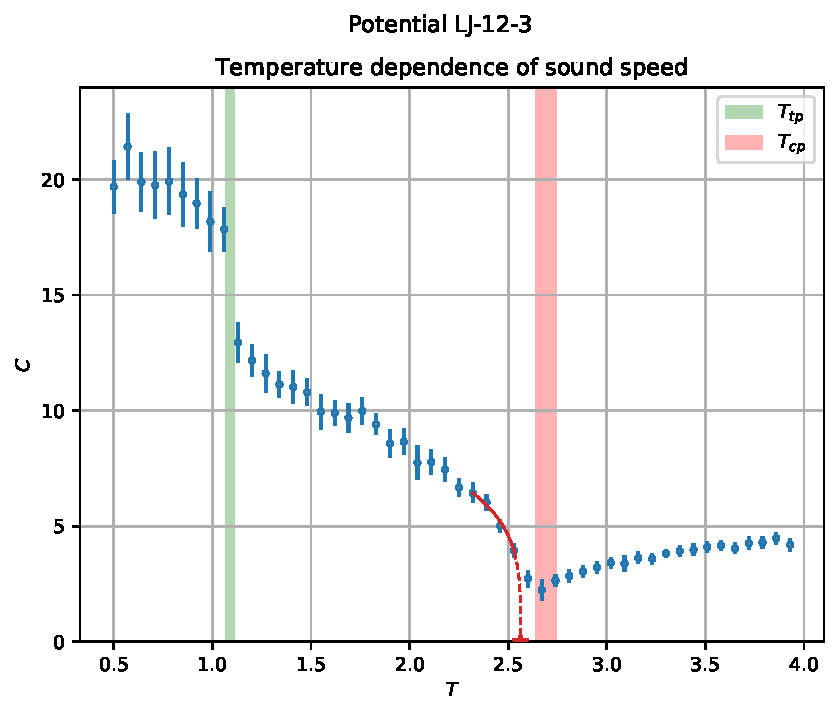
\includegraphics[width=\textwidth, keepaspectratio]{sound_speed_Potential LJ-12-3_1}
\end{minipage}
%\hfill
\begin{minipage}[h]{0.45\linewidth}
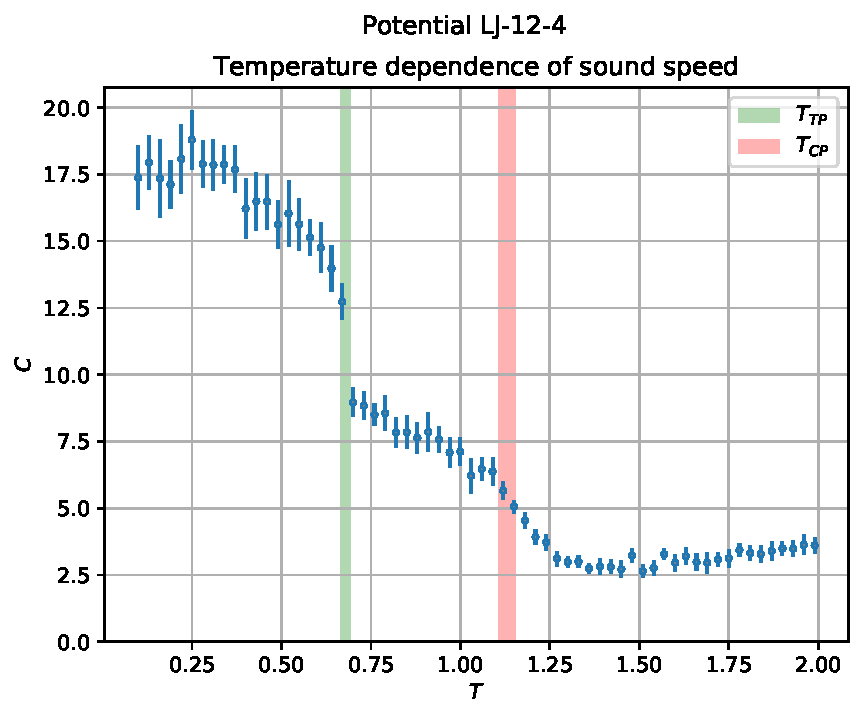
\includegraphics[width=\textwidth, keepaspectratio]{sound_speed_Potential LJ-12-4_1}
\end{minipage}

%\vfill

\begin{minipage}[h]{0.45\linewidth}
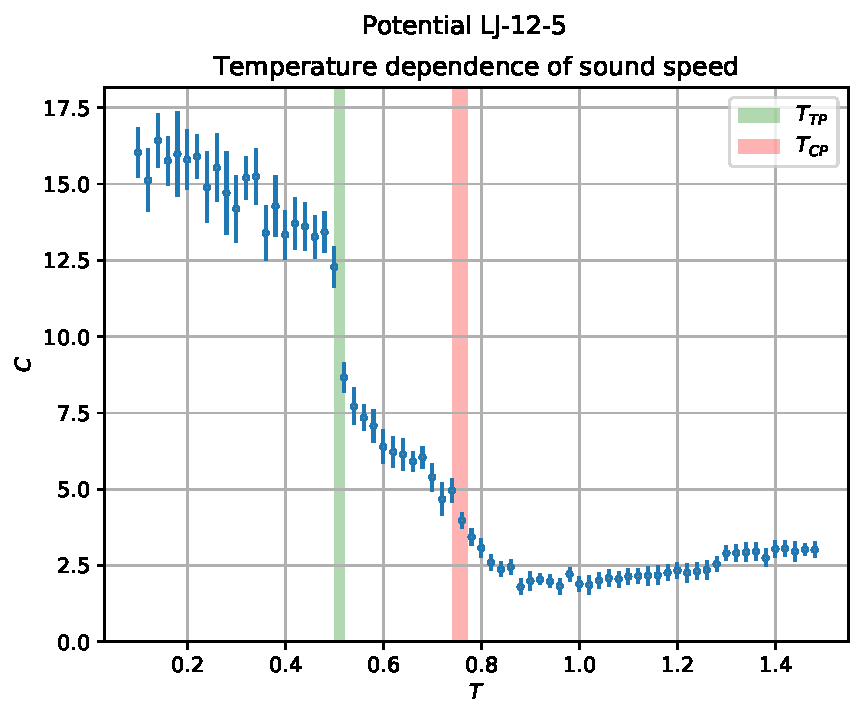
\includegraphics[width=\textwidth, keepaspectratio]{sound_speed_Potential LJ-12-5_1}
\end{minipage}
%\hfill
\begin{minipage}[h]{0.45\linewidth}
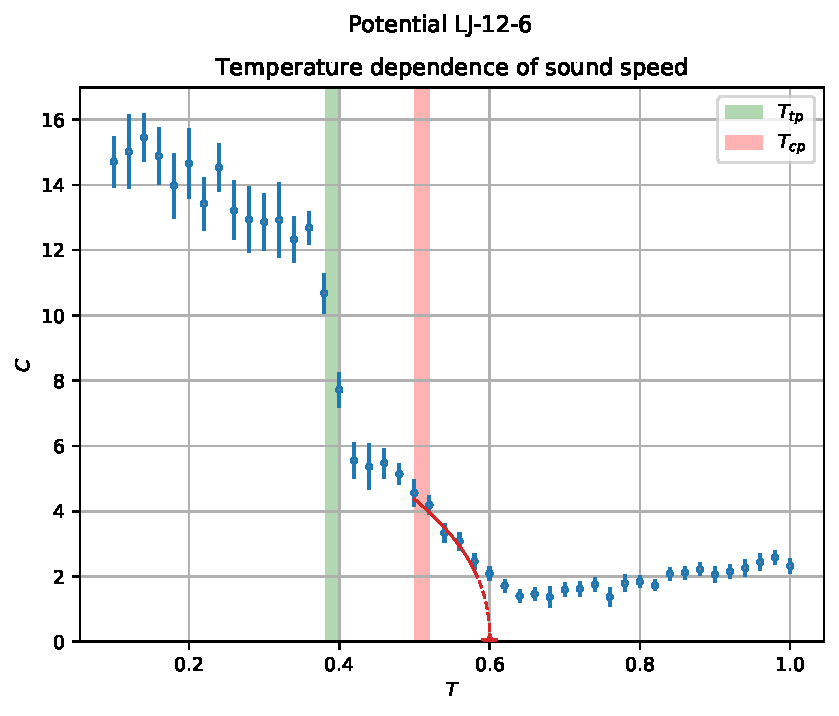
\includegraphics[width=\textwidth, keepaspectratio]{sound_speed_Potential LJ-12-6_1}
\end{minipage}
\caption{Температурная зависимость скорости звука в веществе.}
\label{ris14}
\end{center}
\end{figure}

Текст

\begin{figure}[htbp!]
\begin{center}
\begin{minipage}[h]{0.45\linewidth}
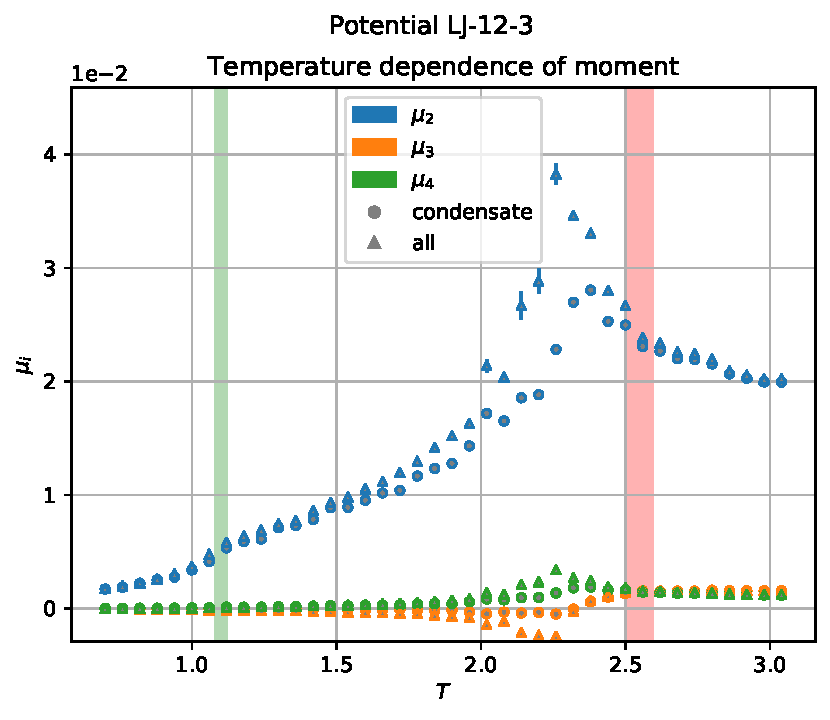
\includegraphics[width=\textwidth, keepaspectratio]{plot_moment_Potential LJ-12-3_1}
\end{minipage}
%\hfill
\begin{minipage}[h]{0.45\linewidth}
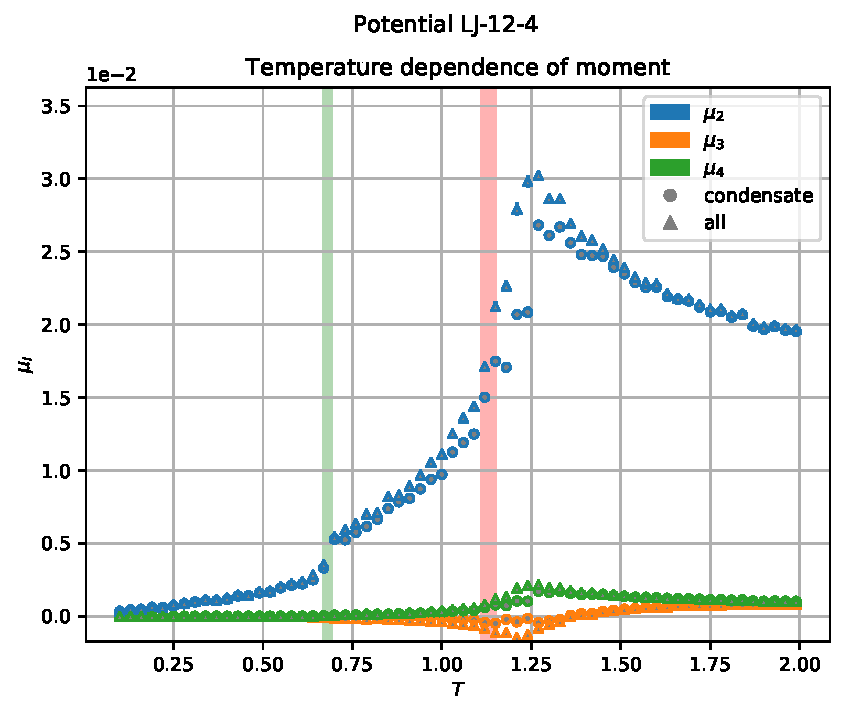
\includegraphics[width=\textwidth, keepaspectratio]{plot_moment_Potential LJ-12-4_1}
\end{minipage}

%\vfill

\begin{minipage}[h]{0.45\linewidth}
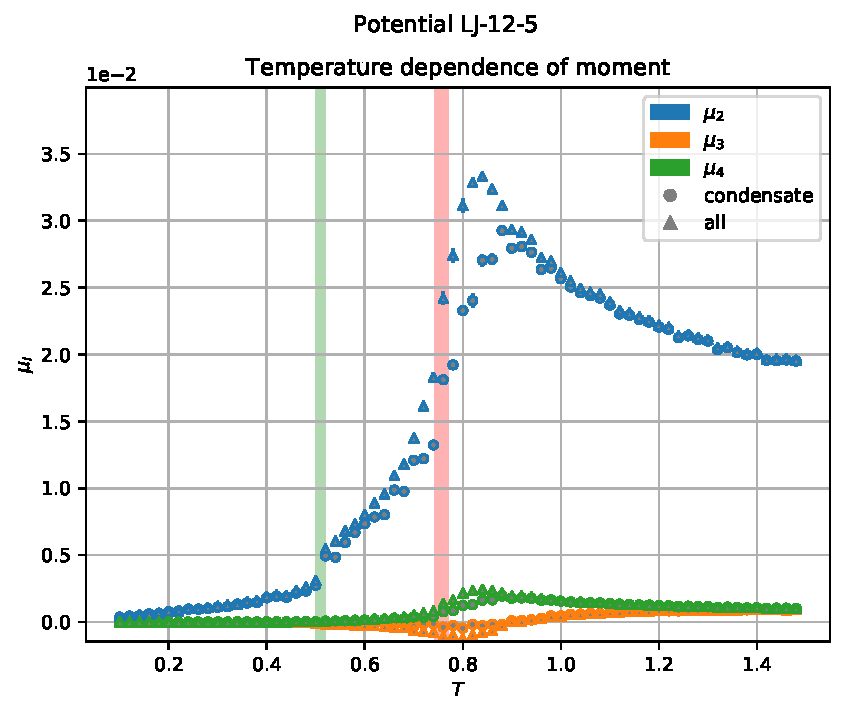
\includegraphics[width=\textwidth, keepaspectratio]{plot_moment_Potential LJ-12-5_1}
\end{minipage}
%\hfill
\begin{minipage}[h]{0.45\linewidth}
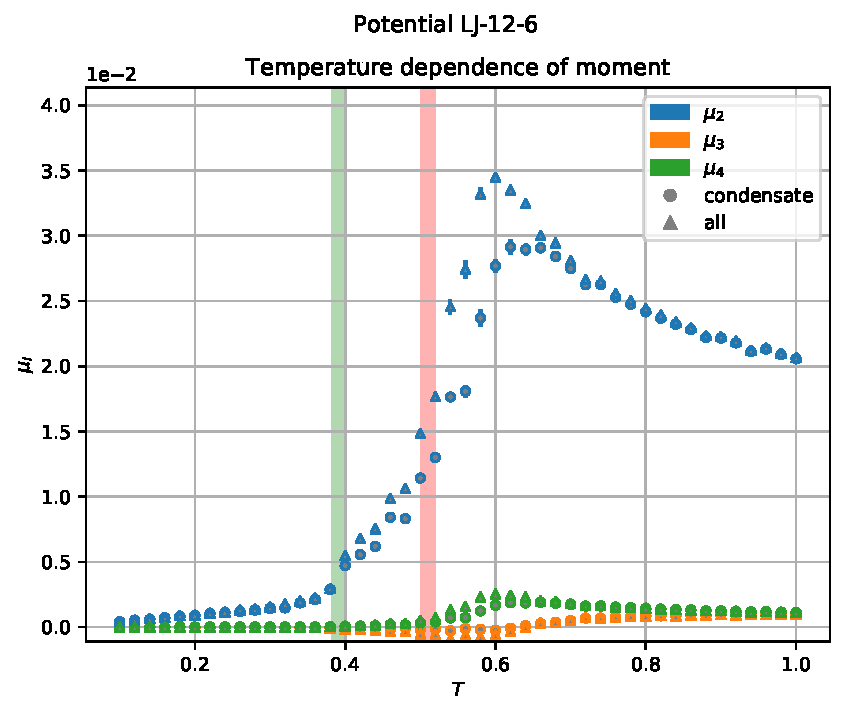
\includegraphics[width=\textwidth, keepaspectratio]{plot_moment_Potential LJ-12-6_1}
\end{minipage}
\caption{Температурная зависимость моментов величины $\mu$.}
\label{ris14}
\end{center}
\end{figure}

Текст

\section{Выводы главы}\label{C2_4}
Вывод.
